\documentclass{beamer}
\usepackage[utf8]{inputenc}
\usepackage{lmodern}
\usepackage[ngerman]{babel}
\usepackage{graphicx}
\usepackage{listings}
\usepackage{hyperref}


\usetheme{Ilmenau}
\usecolortheme{beaver} %ich weiß nicht mehr, ob warsaw standart orchid ist
\setbeamercovered{invisible}
\beamertemplatenavigationsymbolsempty %drecks command, macht die Navigationsleiste weg

\title{Thread-Support und Scheduler für Arduino Due}
\subtitle{Entwicklung von Multithreading-Support mit Präemptiven Scheduling}
\author{Arne Struck}
\institute{Universität Hamburg, Fachschaft Informatik, Abschlussarbeitenseminar}
\date{15.04.2015}

\begin{document}
\begin{frame}[plain]
	\titlepage
\end{frame}

\begin{frame}{Gliederung}
	\tableofcontents
\end{frame}

\section{Arduino}
\begin{frame}{Arduino Due}
\begin{figure}[h]
\begin{center}
	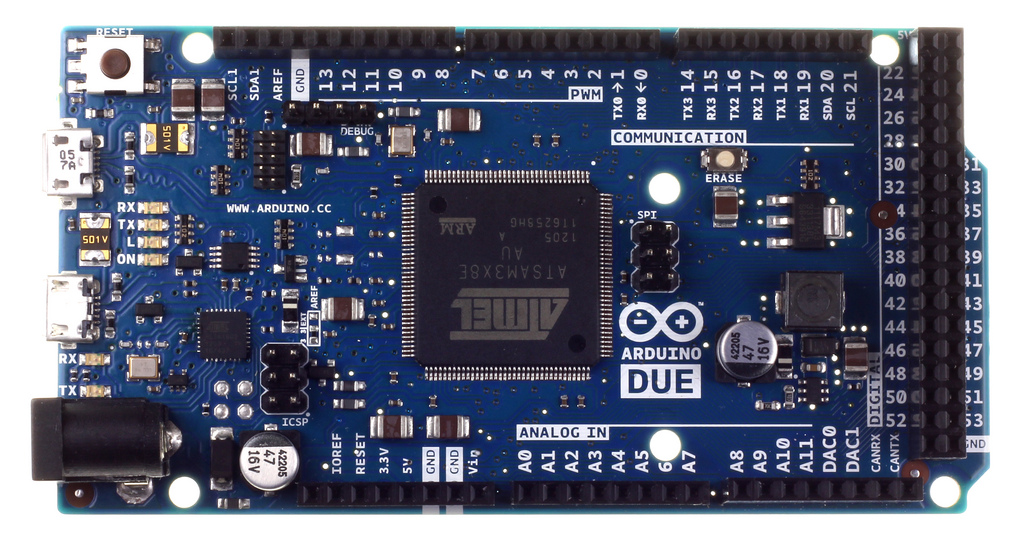
\includegraphics[scale=0.25]{pics/ArduinoDue_Front.jpg}
\end{center}
\caption{Arduino Due (found at \cite{arduinoDue})}
\label{pic:ardDue}
\end{figure}
\end{frame}

\begin{frame}{Relevant Specs}
	Specifications nach \cite{arduinoDue}:
	\begin{itemize}
		\item 32-bit ARM core microcontroller
		\item Flash Memory: 512\,KB (2 Blöcke á 256\,KB) für Nutzer-Software
		\item 96\,KB SRAM (2 Bänke á 64\,KB und 32\,KB)
		\item Clock Speed 84\,Mhz
	\end{itemize}
\end{frame}

\begin{frame}{Done so far}
\begin{itemize}
	\item Beschäftigung mit Arduino Building-Chain \uncover<2>{(WAS ZUR HÖLLE?!)}
	\item<3-> Beschäftigung mit einem bestehenden Ansatz (ohne preemptive Scheduling) \cite{ardMthreading}
\end{itemize}
\end{frame}

\section{Außerhalb}
\begin{frame}{Done so far}
\begin{itemize}
	\item \LaTeX und Beamer Themes, Styles und Möglichkeiten (hier Ilmenau mit beaver) angesehen
	\item Redmine angesehen (Project creator Seite)
	\item repositories angelegt
	\item[$\Rightarrow$]<2-> ("Verwaltungs-") Overhead aufgebaut
\end{itemize}
\end{frame}


\section{References}
\setbeamertemplate{bibliography item}{\insertbiblabel}
\setbeamercolor{bibliography item}{parent=palette primary}
\setbeamercolor*{bibliography entry title}{parent=palette primary}
\begin{frame}[shrink=10]{References}
\nocite{*}
\bibliographystyle{alpha}
\bibliography{literature} 
\end{frame}

\end{document}